\Chapter{LITERATURE REVIEW}\label{sec:RevLitt}
Performance is an important and challenging aspect of the development of software and web applications. Some of the challenges aspects relies in distributed and many core systems, which increased the computational power and the complexity of those systems. In this matter, complementary tools such as profilers and tracers, need to be used in order to minimize their influence in real systems measuring their behavior. Those tools and methodologies are used on performance analysis with different aims. \\
This chapter provides a inside of tools and methods in terms of collecting and analyzing performance data, it also describes techniques for comparing traces, manual and automated analysis of tracing. Finally, the required knowledge to understand deeply our solution is presented in this chapter.\\
Following this schedule, useful techniques and tools for tracing will be presented in section 2.1 through section 2.6. Then analysis methods are presented, classified as automated and manual methods. Later, the current challenges in tracing analysis and the dynamic data structures will be presented. Finally, the proposed solution is introduced.\\
Overall this part aims to present the tools with critical judgment the current data mining techniques and how they apply to this research.

\section{Static analysis and dynamic analysis}
There are two generic and complementary kind of tools to investigate software issues: static analysis and dynamic analysis, below we discuss them with more details. Each of those tools have strengths and weaknesses.\\
The first kind of analysis, static analysis, presents tools that use source code and documentations for their evaluation. Those methods include source code analysis tools \cite{source_code_analysis} and other tools such as \cite{better_code_hub}\cite{Jackson1994SDT645543655704}.\\
There are several ways to statically analyze a code, according to \cite{ind_perspective}, the two main characteristics of static evaluation is the nature and the depth of the analysis. Source code analysis tools include several tools such as Semantic Diff, Better Code Hub and FindBugs. \\
The second tool, Better Code Hub, \cite{better_code_hub}, does a complete analysis of several aspects of the source code of applications focusing in quality measurements and code metrics. The tool uses also definitions of guidelines for code maintenance, such as writing small units of code and doing automated tests.
Although not scanning the code itself, but the bytecode, another tool is FindBugs, \cite{find_bugs}, which does a comparison in bug patterns. It requires compiled class files to find the bugs from patterns and it creates a scale in the possible bugs, from one to four, where one is the worst from the comparison of the patterns. The reported false positive rate is about 50 percent \cite{find_rate}, also this tool has several configurable settings such as finding specific FindBugs does not find all bugs, since context sensitive bugs and security bugs, which involve dynamic behavior of software are not tracked.  \\
Some tools use pattern languages to describe bugs, as PMD \cite{pmd_tool}. PMD uses a set of rules predefined in classes, examples are Double Checked Locking pattern and Unconditional If statements. \\
Static analysis however, is limited for the code and consequently is not able to reproduce exactly the behaviour of very complex and multi-threads systems. 
Another kind of software analysis that can be done is dynamic analysis, basically operate by executing a program and observing (and recording ) the executions. The analysis this runtime data and can be used on performance evaluation for example, but also for software testing. Example of dynamic analysis tool are debuggers, profiler and tracers.\\

\section{Profilers}
The first kind of tools, Profilers, allow to verify where the program spent its time and which functions called which other functions (call hierarchy) while it was executing. This information can be used to demonstrate the fast and the slower parts of code and improve the performance of the application.
An example of profiler is a call graph profiler that show the call times. Gprof is a profiler of GNU GCC tool. Gprof was originally proposed to help the user to evaluate alternative implementations of abstractions.\\
Gprof presents a call graph of the application, which represents the caller-callee relationship, also showing the number of times that it was called. The implementation in gprof uses the mcount which is responsible for creating a table using the stack frame of the application.
Another tool called OProfiler, is a set of monitoring tools related to profiling. It was implemented using a script called opcontrol and a daemon called oprofiled and is able to collect information for all parts of the system: kernel, shared libraries and binaries \cite{oprofile}. This tool uses a mechanism called differential profiles that is able to compare profiles by percentage and has the declared overhead percentage of 1 to 8 percentage impact.\\
However, profilers add a considerable amount of overhead on the system because of the requirements of the code that need to be instrumented. The process to analyse the data is apart from the running part itself in those tools, and the distribution of the functions does not necessarily might reveal relevant information from the execution.\\
\section{Debuggers}
The second kind of tools, debuggers, enable a source code analysis during the execution and aid to understand another program execution. This is done by adding debugging points at arbitrary points of the code, such as when the program crashes.\\
One example is GDB, a debugger the Gnu tool to debug and supports several languages, such as  C and C++. GDB starts as a separate server process and executes the user command. 
There are three kinds of breakpoints in GDB: breakpoints, watchpoints and catchpoints, all of them involving stopping the normal execution of the program \cite{gdb_breakpoint}. The process of debugging is to watch the behavior of those breakpoints analyzing concomitantly the source code of the application.\\
Debuggers, however, increases considerably the overhead of an application because it needs to stop the execution of the application when a certain condition occurs, since this kind of analysis requires a precise addition of the breakpoints in the code. Also since they present a snapshot of the application, they can not find complex interactions component issues \cite{multicore_system_debug}. Finally GDB, as it is primarily designed for fixing bugs rather than tuning performance. \\
\section{Tracing}
Among the current dynamic analysis tools, tracing is a technique that has low overhead and consequently can be used to measure with accuracy several properties of the application, such as its performance.  Different than logging, which deals with high level record of the system, tracing records the low events of the system. This record can then be used for another analysis mechanism \cite{desnoyer}.\\
Tracing can be classified in two main aspects: its functional aspect or its domain of use. The first aspect, the functional, states that tracing can be done in static or dynamic ways. The first, static tracing, requires source code modification and recompilation of the target binary/kernel. In comparison with dynamic tracing, which inset the tracepoint directly in the running process or binary.\\
Tracing can also be divided in the two domains of use: userspace applications and kernel applications.
The first domain, userspace, concerns where the user executes its applications, i.e. The portion of memory in which user executes its processes. In this domain, the system calls can be recorded.\\
The later domain, kernel space, concerns where the core part of the system, the kernel, executes its procedures and the users applications can be traced directly. In this domain, several tools, such as LTTng, already present tracepoints in the kernel code.
\section{Tracepoints}
Tracing involves the addition of tracepoints in the program to measure its behaviour.  Each tracepoint is associated with an event and can be used to record the behavior of the system without the need to create new tracepoints in the source code.\\
In this way, there are two types of tracepoints: static tracepoint or dynamic tracepoints, \cite{desnoyers}.\\
The first type, dynamic tracepoints, are a way collect data in a non-disruptively way. Linux has had dynamic trace functionality for a long time in the form of probes, kprobes, jprobes, and kretprobes. By using probes it is possible to enable to dynamically trace the kernel and consequently, collect debugging and performance information non-disruptively \cite{Yanok2015TLV28183022818303}.\\
Kprobes, specifically, provide a kernel API for placing probes on kernel instructions and they can be exploited directly via a kernel module, or via systemtap which provides a high level scripting language. Kprobes basically is a set of handlers to be placed in a specific instruction address \cite{kprobes}, where a post-handler and a pre-handler is defined. The handlers can be used for multiple probes. The process is the defined as follows: when the instruction is executed, the pre-handlers are executed before the execution while the post-handler are executed right after the execution of the instruction. Also it is possible to use GNU debugger (GDB) tracepoints to insert dynamic tracepoints in the system \cite{sucha_tracepoint}. \\
The second type, static tracepoints, use the already present static tracepoint in the Linux mainline for collecting data. There are several ways to use the static tracepoint via commands or in kernel modules.  Usually static tracepoints are faster than dynamic tracepoints \cite{giraldeau-ols2011}.\\
\section{Tracing tools}
From the kernel space, as described above, the tools are the following: LTTng, Perf, eBPF and Ftrace.\\
The first, LTTng, Linux Trace Toolkit Next Generation, proposed by Desnoyers and Dagenais as a tracer to extract information from the Linux kernel, user space libraries and from programs by running a recompiled instrumented version of the kernel. It was created to aiming for a minimization of the impact of the instrumentation in the kernel,\cite{Montreal_thelttng}.\\
LTTng main components are the daemons, the session and a ring buffer. The session daemon is responsible for interface with the sessions and the overall component control, while the second, consumer daemon writes the data to CTF traces. The session is the communication way between the user and the session daemon, enabling multiple records at same time. Finally, LTTng uses configurable circular buffers, which have configurable features for recording the kernel events and can be tuned according to the user needs, the ring buffers are controlled by a channel.\\
LTTng provides three main modes for tracing recording: normal, snapshot and live mode \cite{lttng}. The first mode is the normal mode, i.e. reading and writing in the ring buffer, by  the sessions and consumer daemons. The second mode is the record of a snapshot of the trace, periodically saved in the buffer and sent to the reading system (relay daemon), the reading system might be in another system.  The third the live recorder mode, where a view system can be used to analyze the information live. Also, LTTng currently is able to trace Java and Python application using similar techniques. The tracing data generated by LTTng is outputted as Common Trace Format (CTF). This format can then be read using Babeltrace or parsed via scripting languages, such as python bindings, \cite{lttng}. \\
The following tool, Perf tools, or perf, is a mainline Linux tools that was developed to measure several software and hardware metrics of the CPU. It is a profiler tool for Linux 2.6+ based systems that abstracts away CPU hardware differences in Linux performance measurements and presents a simple command-line interface. Perf is based on the perf events interface exported by recent versions of the Linux kernel. This research uses the perf tool through the construction of the dynamic data structure to measure the system behavior. \\
Its use has subsequently been extended to interface with the macro TRACE\textunderscore EVENT() and therefore read the Linux kernel trace points. It is possible to use it to generate statistics on the number of times a trace point is executed, for example, or to analyze the number of events that a processor will have been recorded during a period. It can be used to record profiles on per-thread, per-process and per-cpu basis in a sampling approach.\\
A new tool that is being used, the eBPF, enhanced Berkeley Packet Filter \cite{ebpf} is being integrated in the Linux mainline and allows several filtering packages but also custom analysis filters to be done, \cite{brendan_ebpf}. EBPF can be used in the creation of low-overhead latency histograms and heatmaps that can be used in detailed performance analysis and through visualization tools it can be extremely versatile. Moreover, this tool can be used to create programs, eBPF programs, which can be attached to kprobes with low-overhead latency and populate the eBPF maps as explained in \cite{ebpf_maps}. \\
Finally, a standard and known tool, Ftrace is a mainline tool for tracing in Linux . It was designed to find the specificities of the operations inside the kernel. It can be used for debugging or analyzing latencies and performance issues that take place outside of user-space and Ftrace uses the macro TRACE\textunderscore EVENT() to function \cite{ftrace_red}.\\
Although Ftrace is typically considered the function tracer, it is indeed a framework of several of tracing utilities in the kernel side. For example, it can be used as latency tracing to examine what occurs between interrupts disabled and enabled, preemption and event analysis. This tracer is used to dynamically trace functions in the kernel debugging kernel details. \\
Another tracer, SystemTap, allows tracing in kernel space as in user space through the use of dynamic instrumentation, i.e. uprobes and Kprobes. SystemTap relies on  a scripting language that provides flexibility to the user and in addition an interactive GUI. To run those scripts, after written, they are compiled into a module and loaded into the kernel. Although this tool has flexibility, it is not suitable for the collection of a large number of number of events in comparison to LTTng.\\
From the userspace side, the following tools can be used:\\
The first tool, LTTng-UST, is the analogous tool of LTTng (kernel) but to the user-space. For this purpose the tool can be used statically in the code by inserting tracepoint or by the use of mechanisms during the compilation phase (by cyg profile). The two possibilities of using this technique, rather by manually inserting tracepoints in the source code or by compiling the source code with modification have limitations. The first method, inserting tracepoints directly in the source code demands time and might not be done in all the functions. The second method, the compilation with tracepoints is limited to entries and exits of the functions and also might not be done in all of them because of the overhead entangled in this operation.\\
In terms of running mechanism, LTTng-UST has a mechanism to avoid returning to the kernel, combining the two parts of the process, the consumer and the producer daemon. The mapped application is responsible for writing into shared memory, which is subsequently read by the consumer daemon. Two processes have been identified at stake in the trace: the application and the consumer. The consumer daemon is specific for user space tracing since it is a different process than in kernel space. The application directly writes the events in memory and consequently does not pass through the kernel of the operating system. \\
Once the reading buffer is filled, it uses a non-blocking control channel to wake the consumer, then change buffer to continue recording the events and then the consumer will clean the buffer in shared memory. This reduces the communication between the consumer and the traced application.\\
In practical terms, LTTng-UST provides an easily way to introduce tracepoints and including them in the code straight or compiling the code with the specific flag -finstrument-functions, which together with LDPreload, can be used to trace entries and exits of a function, similar to a profiling mechanism.\\
Another tool for userspace, Perf, can be used directly on the user space code, where the counters are placed straight in the code through the use of a library in the source code, the performance counters are then called from it. In this approach the performance counters can be recorded in a sampling approach, where the delta of the beginning and end of an execution need to be computed. This tools is extremely diverse and is able to measure many metrics of the system, software and hardware wise, including instructions, page-faults, cache-misses and so on.\\
Another tool from the userspace domain, uftrace developed by \cite{uftrace} is also a tool that can be used to trace and analyze execution of a program written in C/C++. It was heavily inspired by the ftrace framework of the Linux kernel (especially function graph tracer) and supports userspace programs. It supports various kind of commands and filters to help analysis of the program execution and performance.\\
Uftrace is able to trace kernel functions also, requesting only the root privilege and the enabling of CONFIGFUNCTION\textunderscore GRAPH\textunderscore TRACER=y, in the kernel.\\
Finally, SystemTap, can be in addition be used for user space tracing, through DynInst, and for tracing in user space it is used a User-space mutator DynInst \cite{dyninst} and using the tool Command Line stap this can be accomplished. SystemTap GUI can be used to edit the scripts. It is possible to add tracepoints defined by DTrace and the traces produced by SystemTap are a plain text.\\
In terms of performance, however, it can be slower than solutions which use static tracing, according to the number of threads, for example LTTng.
There are other tools for tracing, apart from kernel and userspace in Linux that are highlighted below:\\
The browser Google Chromium, which is a very known and used tool throughout the world has this feature. The browser provides a method to trace its application and analyze its performance, using an embedded tracing system \cite{chromium_project}. This is a complete solution at the application level, that is tracing and analysis tools, and independent from platform.\\
The tracing mechanism is split in two: tracing recording and tracing consumers. Telemetry is a tool that can be used to trace this application and analyze it, i.e. produce the traces while Chrome DevTools application is a way to consume it \cite{trace_chromium}.\\
The advantage of this technique is portability, since it works independently of the operating system or version. However, the portability of this system, due to its Java Script interface and size limitation for the tracing data, which uses ofIs. As for the chromium traces, they have a limited size and up to few seconds containing only a small number of events. Moreover, the sampling rate in the Chromium software may also cause issues in the analysis of its data, mentioned in our work \cite{google_releases}.\\
Although related to cloud tracing, end-to-end tracing tools have been developed for quite some time. This technique basically enables the tracing of a request from the client-side to the back-end, as defined in \cite{sybase}. End-to-end tracing tools have been widely adopted by several companies as summarized by \cite{mace_list}.
Among those end-to-end tracers, a useful tool is X-trace, \cite{Fonseca2007XPN19734301973450}, which is a diagnose tool tracer and works through metadata insertion, aiming to target all nodes at a network operations. The main purpose of this tool is to reconstruct the task tree of the task of all sub-operations making up the initial task, that is, the set of network operations the observed task has. This is done by adding metadata in the application, this information is disseminated through the nodes of the application to measure it. X-trace has several scenarios of application, such as web servers tracing. This tool is important to highlight considering the several diagnose mechanisms that require end-to-end instrumentation, such as Spectroscope.\\
\section{Challenges in tracing analysis}
The use of tracing for performance analysis can be extremely efficient and feasible, in terms of collecting and analyzing data. However, it has some challenges regarding three main aspects: the size of the trace, the complexity of the data and the analysis of the data. Those aspects are discussed below:
The first challenge is related to the the amount of data generated using the tracing data. This comes from the fact that tracing can record events at low level and, consequently, many events are generated at kernel level \cite{giraldeau-ols2011}. This amount of data can not be easily used compared or analyzed and even with pattern finding or comparison mechanisms. Although some aspects of pattern matching can be improved has emphasized by \cite{similarity_based}.\\
The second challenge related to the analysis of tracing data is the inherent complexity of the data \cite{giraldeau-ols2011}. Since the data converges many aspects of the system, the number of event may require a couple techniques to be applied and mining information from the enormous amount of data. The frequency of occurrences of some events in system plays also a role in the challenge, e.g. an event happening once in a thousand times or more, and consequently some techniques such as pattern mining might not be adequate in all situations.\\
The last challenge resides in the difficult to analyze the cases, since a deep understanding of the underlying mechanisms of the system are necessary. For some performance issues the root cause of the problem is unknown and to profile all the application may not be trivial, thus tracing can be used. The main point in this issue is to find straight association with a singular and specific cause in the trace data with the source code modification that triggered that. For this challenge, a high level data structure, such as a call graph or calling context combined with performance data might be used \cite{doray_article}. 
\section{Performance Metrics}
Hardware and Software performance metrics can indicate key information to describe the state of a system \cite{brendan_book}. Two examples of metrics are latency and throughput. The first can be used to describe the response time of an application, that is it, the time for any operation to complete such as a database request. The second metric, throughput, is the rate of work performed, for example the number of users in a web request.\\
System resources can be measured through hardware and software metrics and the performance of the application that uses those resources can be measured indirectly. System resources might include physical components such as the CPU, memory, disk, caches and network. But, also virtual components such as the network connections  for example sockets, locks, file handles or descriptors \cite{brendan_book}. \\
From this detailed information about the system, such as process scheduling and memory management, it is possible to abstract and control several behavioral aspects of an application as well as the system. Several utilities, as top, ps and htop, can display such information live from the system and used by system administrators to measure the behavior of a system.\\
In terms of tracing technique, performance metrics can be recorded using a special recording mechanism that records the performance metrics using perf\textunderscore events directly in the system. In this case, the metrics must be defined a priori to be enabled in the tracing environment. Besides recording by this approach, it is also possible to use the system dump to record the metrics of the system as they are that recorded. \\
Through the utilization of the approaches described above it is possible to solve performance issues by correlating events with its performance metrics or even with the state of the system.
\section{Performance Anomalies}
There are several classifications for software anomalies, one of them is classifying in three kinds \cite{Chandola2009ADS15418801541882}, others consider four kinds of anomalies \cite{Ibidunmoye2015PAD28086872791120}. The anomalies can be point anomalies, collective anomaly and contextual anomalies.\\
The first kind of anomalies, point anomalies, represent an outline point in the expected values of an application. This definition is broad and might consider a statistical metric as measurement of distance from the mean, for example,  one standard deviation from the mean an anomaly, or more. Those kinds of anomalies might be the spikes in one application that might not affect more than one execution, but will impact considerably the impacted execution.\\
The second kind, collective anomalies, are anomalies that occur not just  once but in groups, i.e. a group of outliers that as a group impact in the application. According to the definition of \cite{Ibidunmoye2015PAD28086872791120}, a special group of those anomaly occur at a frequent time, and consequently have a pattern. \\
Finally the last kind of anomalies are the anomalies that occur because of the context of the application, called contextual anomalies. For those anomalies can be system problems as  IO-bound or CPU-bound. Contextual anomalies are related intrinsically with the infrastructure of the application.
\section{Trace analysis}
There are different techniques to analyze trace data, there are two possibilities of tracing techniques, they are detailed below.
\subsection{Manual Analysis methods}
There are mainly three way to analyze trace data, they are explained below:
The first, using sequence detection, which includes pattern matching techniques, was used in several ways in different contexts. Most of the aforementioned tools use this technique to detect repeated contiguous parts of trace events and to generate abstract and compound events \cite{Pinpoint}. \cite{Fadel}, and Matni and Dagenais \cite{matni} use pattern matching technique to generate abstract events from the LTTng kernel trace events. Pattern matching can also be used in intrusion detection systems \cite{pattern_matching_intrusion}. Some language features are used for matching in OCaml as described by \cite{ocaml}.
For example, STATL, in \cite{statl} models uses signatures in the form of state machines, while in \cite{tracecompass}, signatures are expressed as colored petri nets (CPNs), directed acyclic graphs (DCA) are used to extract security specifications. \cite{behavior_abstraction} present an approach for malware detection using the abstraction of program traces. They detect malwares by comparing abstract events to reference malicious behaviors.Although not related to tracing, in \cite{Fredrikson2011} it is used a behavioral diagnose technique using an algorithmic approximation matching approach, which is a NP-complete, which can be understand as similar to Matni's idea. In addition, a similar approach was explored by \cite{Fournier}, where analyzing blocked processes on multi-core systems, the work was implemented in the former LTTV as Delay Analyzer.\\
However, from all those techniques explained above most of these pattern-matching techniques have defined their patterns over trace events and did not consider using the system state information. Our work is different as, unlike many of those previous techniques, it considers the system states information and provides a generic abstraction framework. Our proposed method converts raw events to platform-dependent semantic events, extracts the system state value, and sends them as inputs to the pattern-matching algorithms.\\
In \cite{naser_abstraction} the concept of trace abstraction aims to reduce trace size and complexity of the data specially for large data processing. In this same work three driven approaches for abstraction are presented: metric-driven, stateful data-driven and a structure-based. Moreover, they were used in \cite{trace_abstraction_1} and \cite{trace_abstraction_2}. While in the first deals with kernel event generation using a semantic approach rather than a low-level representation modelling a state, the second paper, aims to deal with statistics in large trace files, using a statistic database of several metrics through a parameter of granularity degree. \\
Moreover, in this article, a metric-driven approach is explored, it is able to provide statistical data, demonstrating the issues related to this approach: first, the difficulty of efficiently computing the system metrics statistics without having to reread the trace events. The second would be finding a way to support large traces. Although the use of those metrics can be difficult, in the work of \cite{debugging_cluster} is able to do so.\\
The approach of using an automata-based comparison, was done by \cite{matni}, and aims to create a FSM  that simulates the behavior of the system. In this work a pattern mechanism is applied and a list of problematic patterns is diagnosed using State Machine Compiler, SMC, language in the description of problematic behavior. A checker verification is done subsequently in a considerable amount of data to find the patterns and explore the false-true implications. In this article the patterns focus in security evaluation and testing procedures. \\
The work of \cite{TraceFile} introduces a declarative pattern specification language to find pattern-matching in kernel trace analysis. In this work, trace abstraction is explored to compact the information in the traces summarizing the important data. For the specification of the language they used ANTLR.\\
However, the pattern matching technique, as explained above, is a limited manual analysis with linear comparison performance. Another problem is the false-true problems that might arise of finding patterns in the traces.\\
Trace summarization is another possibility to analyze trace data highlighting key aspects of large traces. The work of \cite{summarizing_traces} was to propose an approach for extracting summaries from large trace that rely on the removal of implementation details. The concept of trace summary is related to highlighting the main aspects of a tracing, where the input of the method is the large trace and the summary will bring only the relevant aspects of it, later the representation can be used to represent the system using UML notation. \\
The methodology was applied in the Weka \cite{weka} and was able to represent realistic aspect if this objected oriented library. The aspects for summarization are based in an empirical study using a qualitative evaluation of the software QNX. \\
However, the problem with this technique though is the need to defined previously the main aspects that need to be summarized in a trace. In this work the key aspects of the summarization were compiled using a questionnaire.\\
Another methodology that can be used to compare traces is the analysis of the critical path of a task. In fact, is to analyze a specific task within the trace and be able to follow its trajectory through the multiple threads that it might be executed.\\
The critical path of an algorithm is a methodology to analyse the tasks that occur in multiple threads. For those problems, it was proposed by \cite{francis_phd} an algorithm that is able to find all the threads that contribute to the total time of an execution. \\
This algorithm efficiently retrieve all execution segments that contribute to the latency of a task using some event properties (the sched\textunderscore wakeup) of the Linux kernel, it is possible to identify the multiple threads related to the specific task. However, this tool does not relate this information to user space functions, which makes it difficult to use for fixing application code and the interactive view is able to show just only one execution at a time. For a group of executions comparison, this is severely restrictive.\\
\subsection{Automatic Analysis methods}
For an automatic analysis of the analysis there are several mechanisms to analyze tracing data. One of these techniques is the possibility to use machine learning and data mining techniques.\\
Spectroscope is another tool that uses statistics and high level abstraction to automate the process of analysis focusing in end-to-end tracing, presented in \cite{categorizing_system_behaviour_raja} and \cite{Sambasivan2011DPC19724571972463}. This tool was designed to find changes in behaviour, not find specific anomalies and it was used to find problems in two versions (or periods) on Google's Ursa Minor distributed software. Specifically for this software, five problems are described. It uses Startdust as end-to-end tracers and it added some overhead on Ursa Minor performance, depending the operation. \\
In its methodology, Spectroscope uses Perl language and MATLAB statistical comparison of no problematic period and a problematic period, also using DOT for the plotting part, as other similar tools.\\
The statistical test done is the Kolmogorov-Smirnov test,  which is a non-parametric test for mutation identification that compares the shapes and distribution of mathematical function and later using a ranking system for mutation identification. Spectroscope uses normalized discounted cumulative gain (NDCG), for the performance evaluation, which is a range (from 0.0 to 1.0). The kolmogorov-smirnov test is similar to the KW test since both are non parametrics tests used for comparison evaluation.\\
\section{Methods for analysis}
For the point of view of analysis technique, we can divide them in two main parts: statistical analysis and data mining techniques. In terms of performance analysis, the use of machine learning and data mining techniques were already done.\\
\subsection{Statistical methods}
From the statistic point of view several possibilities of parametric and nonparametric tests can be done such as Confidence Interval, ANOVA and Kruskal Wallis.
The first method, Confidence Interval, which is a comparison of samples considering a percentage of tolerance. This can be seen as similarly to a t-student test.  This method delivers a move from a  relative value estimate to a scope of qualities that are thought to be acceptable for the population. The length of a confidence interval in light of a sample measurement is relies on its Standard Error(SE), which in its turn, depends upon two metrics: the sample estimate and the standard deviation.\\
In co-authored work, \cite{google_releases}, we did an analysis on the confidence interval of several Chromium releases data to find performance regressions. The technique was able to find specific regressions in versions ( specific version data) . This technique can be applied for more uses cases and can be extended to include other technique, such as clustering the data in a previous phase.\\
The second method, ANOVA, can be defined as a way to determine whether there is any statistically significant difference among means of groups of comparison. This technique is used in several areas of knowledge and has different approaches, including the MANOVA and Multi ANOVA.\\
Finally, the third method is the Kruskall Wallis, which is also called anova by rank, which compares medians instead of means as ANOVA. This method is a non-parametric method to compare groups although does not take in consideration most of the assumptions of the ANOVA method.
In performance analysis the use of ANOVA to compare executions was done in \cite{rigorous_statistical}. In this work, the comparison of executions of Java garbage collector, which has problems related to the different behaviour patterns that it can have. This problem based in many aspects of the JIT-process that influence the performance garbage collector problem. Although an empirical study, this work also focuses in the discussion of non rigorous statistical deductions which can occur in the analysis of similar problems. \\
Nonetheless, in our experiments part of the executions did not generate a normal distributed data and consequently the application of a parametric method, such as ANOVA. This is a major drawback that real data might face and that is the reason for applying other methods such as Kruskal Wallis, technique that we explored in \cite{KW}.\\
The work \cite{50}, which implements the tool Pinpoint, builds runtime paths of applications to manage failure for large distributed systems. The tracing is done in the through distributed black-box components until service completes and is able to discover structural anomalies comparing the probabilistic context free grammar, PCFG, of the requests.The comparison mechanisms uses ANOVA and other non-parametric comparison algorithm. The construction of those paths allows the comparison with normal and abnormal paths. Interesting to highlight that in this work, the solution is a combination of three parts and the tracing part is just one part of it, consequently the solution could be used using other tracing scheme.\\
In terms of profiling comparison, the work of \cite{process_control} propose a statistical approach for detecting performance regressions using control techniques. The approach is done by building a linear equation which linearly estimates the number of performance counter samples. The statistical approach is used to compare the predicted and the real counter value using Spearman correlation and for the evaluation it is used the Shapiro-Wilk test. The Shapiro-Wilk is an hypothesis test that assumes as null-hypothesis that the population is normally distributed, as defined in \cite{shapiro}.\\
\subsection{Data analysis techniques}
From the data mining aspect, which is about solving problems using the analysis of data already saved \cite{data_mining_book}, several techniques can be used to find regressions and improve performance.  Machine learning different tasks are cluster and classify the data. The tools to execute them include clustering techniques, decision algorithms and bayesian networks.\\
A common task in machine learning is to cluster the data, also called cluster analysis. It can be defined as separating the data in groups that might not be labeled, support vector machine is one algorithm used in this kind of task. In clustering algorithms, the output will be in the form of a diagram of clusters of data.\\
The first technique, the SVM, support vector machines, is a classification tool in data mining algorithm used to classify the data using a hyperplane. This algorithm requires a learning phase and might be applied to more than one dimension in terms of classification. Another technique is the hierarchical classification algorithm called agglomerative clustering, which cluster the data in a dimensional aspect.\\
This tool was used for performance analysis in \cite{brain} and \cite{constellation}. The first work\cite{brain}, called the Brain, is a dynamic analysis tool that cluster source code to investigate the behavioral aspects of the application. The mechanism was developed as a visualization tool of runtime interactions and was inspired by neural images. This work is related to Execution Murals, which is a way to display runtime interactions of software.\\
In terms of visual cluster, the second work \cite{constellation}, created the Constellation visualization, combines dynamic, run-time information is used to augment the static program model. The tool, is able to do a clustering mechanism by system dependence graph, SDG, at statement-level. The tool combines dynamic information from testing tools which impose low runtime overhead. This works improves the visualization scalability of SDG, which are not so often used, due to the scalability of the current tools.\\
Other tool, Magpie\cite{magpie}, defined as an automatic tool chain for analyzing system’s workload, applies a behavioural clustering technique in system request, considering the resource consumption's and other resources through a stochastic context-free grammar, SCFG. This tool works by analyzing the requests with state machines and then building stochastic workload that simulate real ones. The clustering part is done using a string-edit-distance metric in the data of the requests. Besides, this technique can be used to detect anomalies also considering causal ordering in the tool which is used to produce a canonical annotation of each request.\\
Another task in machine learning is to classify the data, i.e. a function that classify a certain data considering its attributes. One of the ways to do this is to use of Bayesian models for the construction of this function in statistical modeling technique. The model basically works by building a set of conditional probabilities for each attribute, that will be subject to Bayes computation for the classification, as elucidated in  \cite{bayes}. \\
The work of Cohen et al. \cite{cohen} uses a supervised probabilistic model called Tree-Augmented Bayesian Networks, TAN, to identify correlations of system-level metrics related to high-level performance. This technique might be able to identify counters that are highly correlated with bad runs. In the matter of this technique, an interesting survey compiling several aspects of it were summarized by \cite{discrete_bayesian}.\\
The third kind of algorithm, decision tree algorithm, is used to produce sequences  of  rules or association which can  be  used  to recognize the classes for decision making. They can work by ranking specifically a series of properties of a group and how they impact in the classification, and are used in different approaches and context. The work in \cite{decision_tree} applied a technique of performance metrics comparison to diagnosing failures in Internet sites.  The approach was used the traces of eBay using C4.5 algorithm and produced two false positives but was able to find thirteen out of fourteen failures in a real use case. The decision tree was compared with an association rule algorithm and was able to outperform it.\\

The table \ref{tab:performance_data_analysis}
 \begin{table}[h]
\centering
\caption{Comparative methods for performance data analysis}
\label{tab:performance_data_analysis}
\resizebox{1.1\textwidth}{!}{%
\begin{tabular}{lllll}
\hline
Method &  Intention & Pro & Cons & Used in\\ \hline
Decision Tree & Classification algorithm & More flexible than k-means & visualization tool  & [65]\\ \hline
Anova & Compare groups using mean & -More than one group -parametric classification & Assumptions that might not be applied & Gwadera et al [2005b; 2004]\\ \hline
Non-parametric technique & Compare Median comparison & more flexible than parametric tests & non-parametric & [104]\\ \hline
Apriori & Mine association rules & Find associations in any abstraction & Can make false associations & X \\ \hline
SVM & Divide the data using an hyperplane & Optimized division of the data & Hyperplane & Hu et al. [2003]\\ \hline
k-means & Segregate the data & Optimal aggregation &K defined &[87]\\ \hline
Percentage classification &Segregate the data &Can lead to just one group &Number of groups not defined &Our work\\ \hline
Bayesian classification & Mine probabilistic rules & statistical classification & outlines might play strong role & Wong et al. [2003]
\end{tabular}
}
\end{table}

\section{Trace visualization tools}
There are basically three ways to visualize the traces.
\subsection{Gantt Diagrams}
As visualization tool for tracing and performance data, the first is TraceCompass, that was developed by Dorsal Lab and Ericsson in the Eclipse environment and aims at the detailed analysis of several aspects of tracing files. TraceCompass is composed of several sub-projects, composed of analysis and visualization, with specific characteristics.\\
TraceCompass supports several features including critical path and call graph analysis. This can help the developer to highlight several aspects of tracings by applying algorithms of comparison and analysis. However, this tool still requires deep knowledge of the system, as well, of the specific strategy to fix an issue.\\

 \begin{figure}[h]
          \center
          \caption{TraceCompass}
            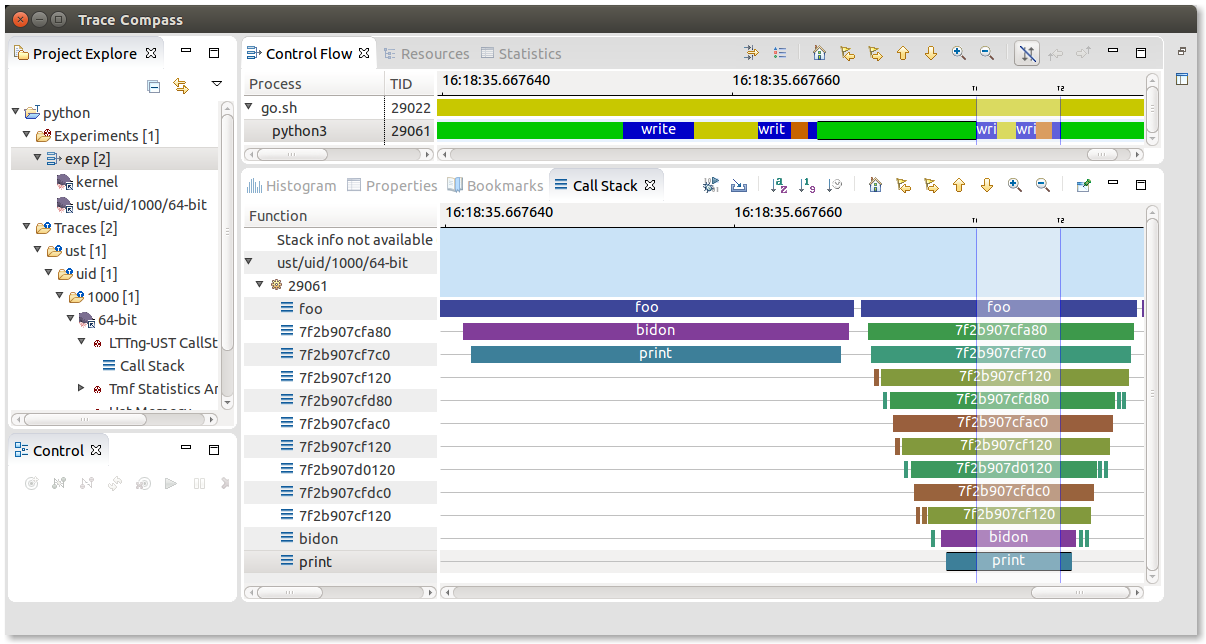
\includegraphics[width=0.90\textwidth]{figures/python-profile-ust-with-kernel.png}
            \label{fig:TraceCompass}
    \end{figure}
    
 
Focusing in real parallelism libraries, the tool Paraver \cite{paraver} is a visualization tool developed by the Barcelona Supercomputing Center. This tool currently traces MPI, OpenMP, pthreads, OmpSs and CUDA. It can be understood as a data browser of parallel traces. In this tool the metrics are programmed, computed from a series of functions and modules. The interesting aspect of  these tools, besides the real parallel traces analysis is the possibility to use programmable definitions to gather the metrics.\\
\subsection{Flame Diagrams}
Another important visualization method, is the Flame Graphs deveped by \cite{brendan_flamegraph}, which is able to show cpu resources and complements heat maps and icicle plots. Flame Graphs are not a tool specifically but rather a methodology of comparison of differences on hot paths in CPU profiling. They can be generated from several ways and originally focused in CPU profiling through linux perf\textunderscore events and might be used to find specifically the function that differ in terms of duration.\\
The tools arrived from the limitations of comparing several CPU profiling the normal tracing and profilers, where those tools could only represent with many lines of text the CPU profiling mechanisms.
Flame Graphs can be used to solve problems such as comparing MySQL data and CPU profiling applications. However, Flame Graphs can face some issues related to incomplete stack traces, function names missing. The incomplete stack traces may lead to incomplete conclusions.\\
A specific kind of Flame Graph, called Differential Flame Graph, DFG’s, is able to compare two flames by using a Red and Green scheme. The original Differential Flame Graphs can challenges in the ambiguity of the color scheme, which has two colors only: Green and Red. This kind of flame graph is used specific to highlight differences in two executions and find bottlenecks in functions of a program's call stack. \\
This methodology requires the full stack trace and consequently some tools might not provide all this information, the stack might also be incomplete or without the symbols loaded. In both cases the stack will be partially reproduced.
 
 \begin{figure}[h]
          \center
          \caption{Flame Graph}
            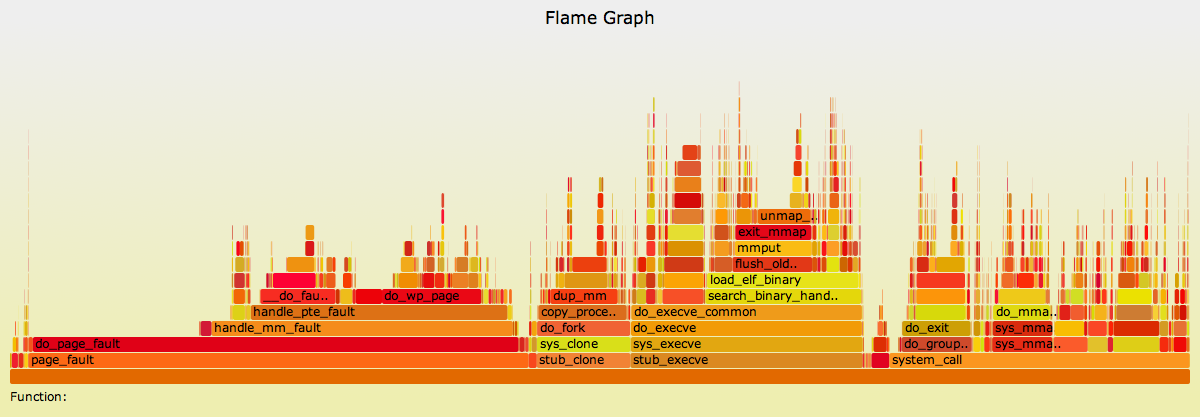
\includegraphics[width=0.90\textwidth]{figures/cpu-linux-execs.png}
            \label{fig:FlameGraph}
    \end{figure}
 
\subsection{Graphs}
In \cite{trevis}, a tool called Trevis, which is a visualization tool related to the calling context tree analysis is presented. It is a visualization and also an analysis framework with a different visualization pattern. It was developed to study the CCT produced from another tool called FlyBy software. It also, as TraceCompare, relies on a calling context tree, CCT, on the caller-callee relationship.\\

Trevis is a visualization and analysis framework that includes several visualization tools such as radial display, TreeMapRenderer, linear  and highrise renderer.
This tool allows the users to play with the Calling Context Trees and applying several methods to compare them. Trevis is able to compare the nodes using many metrics, such as Tree Edit Distance and Multiset Tree Distance. A dissimilarity matrix can be created to compare the similarities of the CCTs and clustering methods can be applied.\\
However, this tool relies in a human interaction and knowledge. Trevis relies on the data from FlyBy profiler tool, to stipulate on the slower executions. FlyBy provides after an report of failure containing this information that later can be used in Trevis to be analyzed.

\begin{figure}[h]
          \center
          \caption{Radial view in Trevis}
            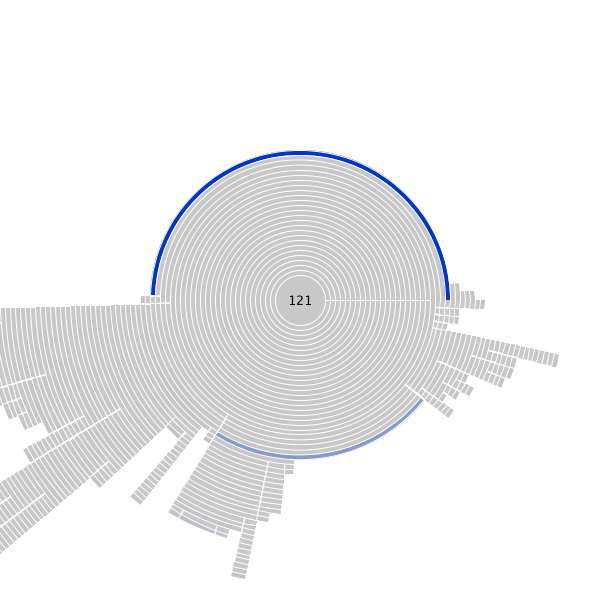
\includegraphics[width=0.60\textwidth]{figures/ring-600-color.png}
            \label{fig:RadialView}
\end{figure}
    
 
\section{Trace Correlation}
Trace correlation has appeared in the literature combining trace from userspace and kernel space. The work of Fournier et al., combines userspace and kernel space data aiming to analyse complex programs in high-level languages, that require userspace tracing, are often written in high-level languages but this work expresses the restriction of availability of those languages. This strategy can be used to compare and find specific differences in the traces aiming to extract more information than just one trace might produce. This is interesting taking in consideration that by using LTTng it is possible to trace them both.\\
In the work of \cite{pattern_based}, a solution that does trace correlation using patterns is used to compare different versions of the same software. The tracers of different versions are compared using a correlation metric, calculated in two approaches. First a non weighted approach, called NW\textunderscore TCM and a weighted approach  W\textunderscore TCM. The solution is composed of two phases, the pre-processing and the correlation calculation, using the already mentioned functions. The work is applied in the Weka \cite{weka} software and was able to correlate the versions 3.4 and 3.7 and found a 70 percent of dissimilarity. However, this technique does not necessarily is easily reproducible since the results require a synchronization mechanism with userspace and kernel space traces\\
Finally, in \cite{thomas}, this technique was also explored for embedded systems, specifically heterogeneous embedded, such as bare-metal CPU. In this work is introduced bare-ctf and it is used traces synchronization techniques. Indeed the solution is applied in Adaptiva Board and presents a generic solution to bare-metal system.
\section{Trace Comparison}
Several tools use the concept of trace comparison to obtain relevant information from the trace data and improve the performance software in general. We highlight here, three of those tools specifically focusing in the the problem definition.\\
One of those tools is TraceDiff\cite{trace_diff}, which does a comparison in the tracing by highlighting their differences. TraceDiff Compares  two  trace files and prints the details of packets that differ to standard output. This is useful for finding packets that are  present  in one trace but not another or for finding conversion or snapping errors. This tools relies in three main characteristic: scalability, robustness and ease of use. \\
However, as the other tools explained above, this tool requires the manual selection of the comparison traces and the analysis of their differences in visual aspects, since it shows the differences visually. The similar traces will be highlighted and connected, whereas the ones diferent will not be in this manner. \\
TraceCompare, was developed in Dorsal lab, \cite{tracecompare}, and it is a tool for performance comparison, it can be used in the two domains: userspace and kernel space. 
The methodology used in this tool is to create a tree data structure, a Calling Context Tree with metrics, from the tracing data to measure the executions of a program and that can have metrics. The segments are defined by the user as sequences of beginning and end, which will delimit the nodes in the tree data structure. The nodes also can aggregate data of the performance in those segments. \\
This tool was developed to compare traces of execution and it uses a javascript front-end and tibeebeetle as back-end. To do this CPU profiling comparison, the GUI tools provide Differential flame graphs, similar to  \cite{differential_flame}. It was able to find abnormalities in the write function of MongoDB after several runs. \\
However, TraceCompare requires expert knowledge and consequently, even after a statically tracing implementation the comprehension of metrics, as suggested in future work, \cite{doray_thesis}. Also the comparison is restricted to two groups and it is manually done. This last characteristic gives an interesting opportunity for further tools, such as our solution. 
\section{Root cause analysis and detection}
In terms of performance anomaly detection and bottleneck identification, PADBI, there is an interesting research currently with some trends. Part of the research is relative to the detection methods, while the other part concerns the identification of root causes, \cite{Chandola2009ADS15418801541882}.\\
In terms of anomaly detection the methods can be defined as detection of monitoring and might or not use data mining techniques. \\
The work of \cite{lasso} presents a Regression-based diagnostic framework for analyzing performance anomalies and potential causes of SLA violations in virtualized systems. Their approach is based in a variant of Least Angle Regression (LAR) called on Lasso, used to identify suspicious system metrics accounting for observed performance anomaly.\\
Another research, \cite{anomaly_detection_grid}, does models the relationship between application metrics and system metrics to explore properties of selection, reduction, and anomaly detection. The approach used combines the use of Fourier transform method, which will provide data to a windows averaging statistical. The use of the Fourier transform is to track patterns in the data.
In terms of root causes analysis several methodologies have been applied to this process. The terms analysis is related to the fact that those tools find the cause of issues.
Using kernel information, the work of \cite{tipme} investigates causes of unexpected long delays in GUI-based user interaction applications. This work developed the collection of tools called TIPME, The Interactive Performance Monitoring Environment. \\
The tool CloudPD,from \cite{cloudPD}, is an example of framework that uses linear correlation analysis to determine variations in Virtual Machines with uses cases like Hadoop and RUBiS. In this work there are several contributions specially in terms of implementation. In terms of root cause analysis the use of correlation-based performance models can be highlighted, although a similar approach was used in \cite{model_prob}.\\
The work of \cite{root_cause} detect anomalies in web applications using an approach called AOP-based monitoring, since it is based in Aspect Oriented Programming. It uses a correlation approach and time-series alignment to verify  the what is the root cause. The root cause analysis is done through a module called Performance Analyzer. This model applies an equation procedure and statistical correlation was done via three correlation methods: pearson correlation, Kendall rank correlation and Spearman Correlation, where the Pearson correlation gave the best results., which requires an alignment using Dynamic-Time Warping algorithm, DTW.\\
\section{Regressions Tests}
Regression testing is performed after making a functional improvement or repair to a program. Its purpose is to determine whether the change has regressed other aspects of the program, such as the performance, \cite{book_testing}. It can also seen as a confidence test proven that the new version works as the previous version\\
The importance of this kind of test is the tendency of adding bug codes throughout the development of updates. It is necessary to do a plan for regression test and before the release of the software, avoiding the deployment of bug code for users.\\
In terms of research at this topic, comparing releases, the work of \cite{parcs}, which developed the tool PARCS, does an investigation in regression tests using CCTs and matching techniques and bytecode comparison. The regressions are done using Apache Byte Code Engineering Library, BCEL. \\
Although not related to performance analysis, in \cite{book_testing}, it is addressed the problem of regression tests in objected oriented code using a comparison of interprocedural control flow graph, ICFG. This paper concerns the test selection problem specific for C++ languages providing a code based technique to in terms of test in the derived class.
\section{Dynamic Data Structures}
In dynamic analysis several data structures have been used to represent the call-caller relationship. The profile data can be either used for code optimization or for general program understanding. The organization of the procedures and its order usually are represented in a call graph or a calling context tree.
The call graph is a useful data representation for control and data flow programs which investigates interprocedural communication (i.e., how procedures exchange information). It contains all the procedures and the relationships among the procedures in a program. A call graph can be represented as a node as functions and edges as call-caller relationships. 
Taking in consideration the context, i.e. the chain of methods up to the root, two main methods are used: Call Trees and CCTs.\\
In the Call Trees, there is an addition of a new node is added for each called method. \\
This data structure can represent with accuracy the complete chain of methods of an application. \\
The other run time structure, calling context tree, CCT, provides flow sensitive profiling data with the nodes was introduced in \cite{blueprint}. In this work the hardware performance metrics from profiling were also taken in consideration in this work. Calling contexts are very important for a wide range of applications such as profiling, debugging, and event logging.  In \cite{blueprint} it is used a call graph to compare executions and explores the so called  performance evolution blueprint.  It is used to track the behaviour evolution of the system.\\
Following the previous work and by using tracing data, in \cite{doray_article}, aggregated performance metrics in a calling context tree to build an enhanced structure that could be compared. In this work it is built a tree with aggregated data, called ECCT, that relates the performance metrics to each node, which represents the functions of the application. This data is later analyzed off-line and, by using the critical path of the task, is able to find differences in the metrics of the ECCTs.\\
In the tool Introperf, \cite{Introperf}, the system stack traces is used to generate a specific CCT, which are called Performance Annotated CCT. In this tree a comparison technique is used to compare the latencies. It was implemented using Windows ETW,developed by \cite{ETW}. In terms of performance root cause, it is explained in the paper about the latency inference algorithm used for this calculation. They used this approach to avoid the requirement of source code or modification to application.\\
Another tool that builds CCTs is PerfDiff, which targets VM’s \cite{perfdiff}. In this work a framework for characteristics of those trees. According to the authors, it is possible to compare the CCT’s in two complementary ways: weight difference and topological difference. The first kind of comparison is the weight difference that is done in two ways: node based weight matching and sub-tree base weight matching. The topological differences are done via common tree matching, which is an algorithm developed by them which states that the nodes match (of each tree) when all the nodes in the path from the root match. This approach is applied to several Java and J2EE applications where the call counter are used as performance attributes.\\
In terms of building the CCT, two main techniques were used previously to collect the stack frames of the application, in the so called stack walking process. The exhaustive approach and the sampling based approach, although other methods such as static and adaptive bursting had been used.\\
When taking all the tracing entries and exists to build the CCT, the result will be the complete tree of the application. The overhead of adding all the entries and exits is a major drawback in this approach.\\
The second main approach is the sampled technique. This technique is able to reduce the overhead in comparison with the exhaustive but has two main disadvantages: inference of calls, which may lead to misinformation and the rate of sampling may not be feasible to a certain extend.\\
Other approaches are possible such as static stack walking and adaptive stack walking. The same authors of PerfDiff, previously proposed the use of Adaptative Bursting technique for the stack walking process in \cite{adaptative_burst}. This kind of stack mechanism avoids the overhead of creating the trees in a process of eliminating certain profile data redundancies.
We also used a version not summarized of the frames with the metrics, and in analogy to the ECCT, the tree was named EDT, Enhanced Dynamic Tree. They are very similar, though the EDT is not summarized and can facilitate the mining process relating each node to the metrics without further calculus. 
\section{Auto Grouping mechanism}
During software execution several parameters might change and the application performance can vary according to many factors. This can occur even when the algorithms used are deterministic and no probability is used. The cause for those variance are outside the scope of the program itself.
However, some applications might have issues in the code, related to its implementation details. Software tests mechanisms might not be sufficient to reveal this behavior especially in terms of performance discrepancies.\\
An example was found in \cite{doray_article}, after executing several times the same query operation on MongoDB, a free open-source database framework, its performance decreases abruptly a further investigation lead to the root cause of this performance issue. \\
The auto grouping technique presented as the solution for those kinds of problem. The approach is to do automatic comparison of executions of the same program in the same configuration settings and investigate their metrics behavior. \\
The solution is automated by a heuristic comparison of several groups distributions and can be applied to an arbitrary number of groups together with a clustering mechanism, such as k-means. The automatic grouping gives the optimal number of groups in terms of SSE and together with a comparative mechanism, can be used to find associations between groups. 
The division in groups enables the comparison and study of their variances using different approaches, for a few number of groups the investigation by the comparison the variances of the metrics of the groups can lead to the discovery of root causes. Another approach can be the use of apriori algorithm which can be applied to find association among the groups. 
The complete solution is able to find associations between the performance and metric variations, i.e. groups of different performances and metrics. This can indicate if a specific metric is responsible for a certain groups of execution that have a bad performance, in a fuzzy approach and that can be applied for infrequent problems.\\
\section{Conclusion of the Literature Review}
In terms of dynamic analysis of an application, tracers, profilers and debuggers can be used, each one with its own specific pros and cons.
Profilers represent the caller-call relationship and allows a deep understanding of the time consumed in an application. Profilers add extra overhead and might not be suitable to find performance issues that occur in group in several execution of software.\\
Debuggers can be used specifically to find a part of code that might trigger issues in the execution. This tool relies in breakpoints that will stop the execution in a specific condition. This process allows specific conditions in the source code to be tests and bug finding and fixing accessible. \\
Finally, tracers use advanced technologies and implementations to record events occurring at several levels in a computer system with minimal overhead. This feature makes tracing a useful mechanism to understand and analyze the behavior of the system in the real context.\\
By using tracing technique it is possible to develop a data structure which represents the dynamic execution of a system but also can be embedded with performance data recorded in the tracing data. Several other techniques can relate this performance data with specific functions in the same node and allows associations of metrics and functions.
In summary, several strategies make it possible to extract from one or more traces all the events related to a given task execution. However, there is a demand for automated tools to analyze the performance.  \\
This research is based on the several methods of comparing performance data that were introduced in this chapter, including data mining technique and statistical evaluations gathered using profiling and tracing mechanisms. In the next chapter, we present the methodology used throughout our solution.\\

\section{Summary of the tools}
The table \ref{tab:tableComparative} summarizes part of the related research.\\

 \begin{table}[h]
\centering
\caption{Table Comparative tools for performance analysis}
\label{tab:tableComparative}
\resizebox{1.1\textwidth}{!}{%
\begin{tabular}{lllll}
\hline
Tool             &    Intention & Pros & Cons & Kind of tool   \\ \hline
PerfDiff &  Generate CCT in VM’s & Node and weight comparison & Topological differences might mislead & Detection and analysis \\
\hline
TraceCompare & Compare groups of executions & Easy to use  & Manual select entries and exits & Detection and analysis\\ \hline
Spectroscope & Distributed system behaviour categorization & Automated k-means & -Time for the analysis -Relies in end-to-end instrumentation  & Detection Analysis\\\hline
Introperf &  Generate CCT & Based in ETW  & -Complete stack walking -overhead & Detection and analysis
\\ \hline
 
Spectraperf \cite{SPECTRAPERF} &  Detection of I/O regressions & Efficient performance Specific for I/O &  Comparison of two software versions & Detection and analysis
\\ \hline
Pinpoint &  Build runtime paths on large systems & Comparison using a free context grammar & ANOVA requires normal distributed data & Detection and analysis\\ \hline
TraceCompass &  Trace Analyze &  Several internal tools and methods & Manual analysis & Analysis \\ \hline 
Magpie & Automatic tool chain builder & Use of a comparative metric: string-edit-distance metric & Probabilistic construction of the event & Detection and analysis\\ \hline 
Trevis &  CCT analysis tool & Manual method & Rely in another tool & Visual method Analysis 
\end{tabular}
}
\end{table}

